\documentclass[../thesis.tex]{subfiles}

\begin{document}

\begin{comment}
What do I want people to know after reading this?

* Modeling is useful because it allows us to understand the physical causes of VI in great detail. It also lets use explore different scenarios.

* Some basic background about VI, such as a brief history of it and indoor air quality (Radon etc).

* What are the current hot topics in VI?
- ITS
- CPM

* Why is temporal and spatial variability a problem in VI?
\end{comment}

\chapter{Introduction}
% TODO: Think about if you want more subsections in background and variability issues.

\import{./}{background.tex}
\import{./}{variability_issues.tex}
\import{./}{proposed_solutions.tex}
\import{./}{problems_with_solutions.tex}
\import{./}{modeling.tex}
\import{./}{outline.tex}





\begin{comment}
\subfile{./background.tex}
\subfile{./variability_issues.tex}
\subfile{./proposed_solutions.tex}
\subfile{./problems_with_solutions.tex}
\subfile{./modeling.tex}
\subfile{./outline.tex}

\section{Indoor Air Quality and Vapor Intrusion}
% History and perspective on indoor air quality
Concerns about air quality are as old as civilization itself, ranging from beliefs that disease is caused by bad air - a \textit{miasma}, to more recent concerns about exposure to combustion particulates, radon gas, or other air-borne pollutants.
Since industrialization the number of potential hazardous pollutants has increased significantly, followed by increased concerns about air quality.
At the same time, people now spend more time indoors now than ever before, with Americans spending up to 90\% of their waking time indoors\cite{klepeis_national_2001}.
This change in human habitation has put a special emphasis on indoor air quality.\par

Some early scientific inquiries into indoor air quality focused on pollutant sources that were generated in the home, e.g. by heating and cooking systems, and these types of pollutants are still relevant today, but of particular concern in developing countries\cite{craig_d._hollowell_combustion-generated_1976,world_health_organisation_who_2014}.
Many buildings materials can also cause indoor air quality issues, with exposure to asbestos fibers being perhaps one of the more famous examples of this.
Mold is another common indoor quality concern\cite{world_health_organisation_who_2009}.\par

% Introducing Rn
In the 1970s, to address the growing public health concerns, research began into the potential exposure to radioactive radon gas in buildings.
Radon gas, which is generated by the decay of naturally occurring uranium in soils and rocks, was found to be able to enter overlying building and expose the inhabitants.
This phenomena came to the public attention in the mid 1980s, after a Pennsylvanian nuclear power plant worker set off radioactivity sensors at the plant, the actual cause of which was the high concentration of radon gas in the workers home\cite{noauthor_health_nodate}.
Exposure to radon gas can significantly increase the risk of developing lung cancer, and is to this day the second leading cause of lung cancer in many countries\cite{gaskin_janet_global_nodate}.
With the discovery of radon intrusion into buildings, it did not take long for the same concerns to be extended to the entry of anthropogenic contaminant vapors - vapor intrusion (VI).\par

Vapor intrusion is the migration of contaminant vapors from a contaminant source, often contaminated groundwater, into the overlying buildings.
These vapors evaporate from the contaminated groundwater and enter through cracks in the building foundation, gaps between walls and floors, sump pits, or other openings\cite{u.s._environmental_protection_agency_oswer_2015}.
In these aspects, VI is more or less similar to radon intrusion, and thus much of the early VI research was heavily influenced by the work done by radon intrusion researchers.
This is largely true to this day, but vapor intrusion differs in some non-trivial ways, that make it an unique issue.
Many of these differences stem from the properties of the contaminants themselves, and from the fact that many of the VI contaminants that we concern ourselves with, mainly volatile organic compounds (VOCs) and chlorinated solvents, are of anthropogenic origins.\par

One difference is that radon is unstable, and has a half-life of around 3.8 days (at least Rn\textsuperscript{222}, the only naturally occurring isotope of radon), and it follows that radon accumulation will be naturally mitigated, which is not the case with other contaminants\cite{schumacher_fluctuation_2012}.
The closest analogy is that certain VOCs of VI concern are able to be biodegraded by bacteria in the soil, but this effect can vary significantly as this process is oxygen limited\cite{u.s._environmental_protection_agency_oswer_2015,abreu_simulating_2006}.\par

A more significant difference is the anthropogenic origin of VI contaminants.
In VI, we often are concerned with a contaminated groundwater source underneath the afflicted building, and the source of the groundwater contamination typically originates from some contaminant spill at one or more sites in the surrounding area.
Thus, a large number of buildings may be impacted by VI via a single contaminant source.
The origins of such spills are numerous, but any activities that employ the contaminants of VI concern are possible culprits\cite{u.s._environmental_protection_agency_oswer_2015}.
In the United States (US), the Environmental Protection Agency (EPA) maintains a list of significantly polluted sites throughout the country, so called Superfund sites, and as of 2020 there are 1335 recorded sites, many of which contain the contaminants of concern\cite{us_epa_current_2015,u.s._environmental_protection_agency_oswer_2015}.
Additionally, many of the contaminants of concern do not readily degrade, and legacy contamination is an issue\cite{u.s._environmental_protection_agency_oswer_2015}.
It should also be noted that VI from a contaminated groundwater is only one type of contaminant source, with leaky subsurface tanks, spills into soils, etc., likewise being contaminant sources of concern.
Figure \ref{fig:vapor_intrusion} shows some of the VI processes.\par

\begin{figure}[htb!]
  \centering
  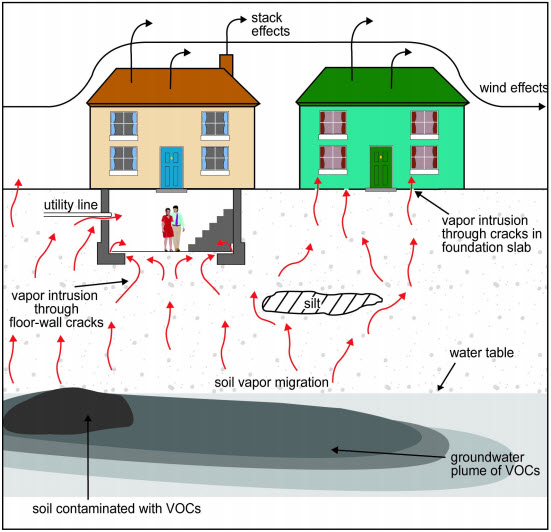
\includegraphics[width=0.75\textwidth]{vaporintrusion.jpg}
  \caption[Overview of vapor intrusion]{Vapor intrusion into a building can occur through a variety of means, from a variety of sources. Figure from the EPA\cite{us_epa_what_2015}.}
  \label{fig:vapor_intrusion}
\end{figure}

In VI, some common contaminants of concern are chlorinated solvents such as trichloroethylene (TCE), tetrachloroethylene (PCE), or chloroform.
Various other organic compounds such as benzene, or other petroleum products are also of concern.
Out of the various VI contaminants, TCE has emerged as of perhaps particular concern.
TCE is an excellent degreaser and has seen extensive use as such, and has been commonly used by dry cleaners, the military, auto repair shops etc\cite{u.s._environmental_protection_agency_oswer_2015}.
The concern over TCE is partly due to its associated cancer risk and partly because it was recently hypothesized to possibly play a role in birth defects.
A review study by \citeauthor{makris_systematic_2016}\cite{makris_systematic_2016} showed that TCE may be associated with increased risk of congenital heart defects (CHD), but a more recent study by \citeauthor{urban_systematic_2020}\cite{urban_systematic_2020} concluded that, mainly due to reproducibility issues and new studies, there is not adequate evidence to support that TCE causes CHD.
Regardless, it is carcinogenic and surprisingly despite the concerns about its health effects, its use remains legal.\par

Considering the widespread existence of potential VI sites and the associated health concerns, an industry for identifying and characterizing these sites and either remediating or mitigating them has emerged.
This is particularly true in the US, where the law dictates that the responsible party of the contaminant spill or release is liable for cleanup and mitigating human exposure.
In this situation significant effort is spent on determining liability.
Determining if VI occurs at a particular site, as we will see in this work, is not easy, and while VI has been studied for decades, many questions and challenges remain, in particular with regards to the great spatial and temporal variability that exist both within and between VI sites\cite{u.s._environmental_protection_agency_oswer_2015}.\par

\begin{comment}
Purpose is to demonstrate the issues that temporal and spatial variability causes in VI site investigations, and impress upon the reader the necessity to solve these.

- State the general issues, i.e. harder to assess real human exposure, more expensive, etc.
- Give examples in the literature and describe the situation. (1-2 examples for spatial/temporal respectively should suffice.)

Topics to cover:

Issues that confound VI investigations:
* Indoor sources/false positives (problem with only indoor samples)
* Sub-surface contaminant formation by indoor (sub-surface samples)
* Groundwater samples (spatial variability & presence of contaminants here does not mean entry occurs)
* Issues with preferential pathways
  * Indie style (long distance transport of contaminants)
  * Kelly style (plumbing fixtures)
  * ASU style (+ Danish study?) (nearby sub surface features that are not readily apparent)
* Seasonal aspect
* Necessity of MLE
  * Expensive and hard
  * Need for more robust methods

\end{comment}

\section{Issues In Vapor Intrusion Investigations}

% Some issues with VI investigations
Determining if vapor intrusion occurs at a building is often difficult.
One might be tempted to believe that collecting an indoor air sample inside the building would be sufficient, i.e. that if the vapor contaminant concentrations is over some threshold in the house, proves that IV occurs, and the absence of contaminant vapors is proof that no VI occurs.
However, this approach is too simplistic and may yield false positives.\par % TODO: Source

% False positives
Many common consumer products contain the same contaminants that is often of concern in VI, and the presence of e.g. a petroleum containing gas tank may be the culprit.
Not all indoor contaminant sources are so obvious though, and many contaminants may be inadvertently introduced, such as by bringing home newly dry-cleaned clothing.
Great care is taken to eliminate such indoor sources, but can be challenging.\par % TODO: Source

A compounding issue related to this (and other topics) is that many of the contaminants can sorb onto/into various materials and subsequently desorb for significant periods of time, potentially extending the influence of indoor source beyond their removal.
This a phenomena, among other related issues with sorption, we will discuss in Chapter (TBD).\par % TODO: Reference chapter later

Since indoor air samples may not sufficiently prove that VI occurs, one usually have to take further steps.
One such is to collect air samples right below the foundation of the building, and if contaminant vapors are found there, as well as in the indoor air, that is more compelling evidence that VI occurs.
However, as work by \citeauthor{holton_creation_2018}\cite{holton_creation_2018} has shown, contaminant vapors in the indoor environment may migrate from inside the building to the subslab, creating a contaminant cloud that may persist for significant periods of time, rendering some extra uncertainty.\par

Collecting samples from the contaminant source, such as the groundwater underneath a building, to determine the presence of contaminants can be used as another potential evidence of VI.
However, even identifying the source alone is not enough evidence as the presence of a contaminant source does not mean that the contaminant vapor enter the overlying building.
\citeauthor{folkes_observed_2009}\cite{folkes_observed_2009} who conducted a decade long study of VI sites in Redfield, Colorado, and a 19 month long study in New York showed that many of the sites, even though they were above a contaminated groundwater source, were not impacted by VI.\par

Often one would take samples from different locations, the types already discussed as well as soil-gas samples, and compare the relative decrease in contaminant vapor concentration from the source to the indoor to determine if entry ultimately occurs from the source.
This subsequent decrease is called \textit{attenuation} and is quantitively determined as an \textit{attenuation factor}, where the indoor contaminant concentration is divided by the contaminant concentration in the soil-gas or groundwater.
$\alpha$ is often used to represent the attenuation factor, and in this work we will often use a subscript to denote attenuation from where.
In the case of groundwater attenuation for instance, one would divide the indoor contaminant concentration by the groundwater contaminant vapor concentration (that is when the contaminant concentration is in equilibrium with air, e.g. Henry's Law).
\begin{equation}
  \alpha_\mathrm{gw} = \frac{c_\mathrm{in}}{c_\mathrm{gw} K_H}
\end{equation}
Where $\alpha_\mathrm{gw}$ is the attenuation from groundwater;
$c_\mathrm{in}$ i sthe indoor contaminant concentration;
$c_\mathrm{gw}$ is the groundwater \textit{liquid} contaminant concentration;
and $K_H$ is the dimensionless Henry's Law constant.\par

Over time, the U.S. Environmental Protection Agency (EPA) has compiled data of attenuation factors relative to different depths and source types.
Using these data, standards as to which attenuation factors are to be expected relative to these metrics have been established to help guide investigators and regulator determine if VI occurs.
This is helpful, but often we are faced with VI sites that render these sort of standards difficult to use.\par

Heterogeneity in soil, distribution of contaminant source concentration, as well as source type (e.g. a contaminant spill in the soil itself or some leaky chemical tank underground), can all contribute to significant spatial variability in contaminant concentration at a site.
A good example of this is a study by \citeauthor{luo_spatial_2009}\cite{luo_spatial_2009} where contaminant concentration beneath a build foundation varied from 200 to less than 0.01 mg/L.
\citeauthor{bekele_influence_2014}\cite{bekele_influence_2014} likewise found that TCE soil-gas concentration could vary an order of magnitude underneath the foundation of their site.\par

Likewise, not all indoor environments are perfectly mixed and indoor contaminant concentration can vary significantly between different rooms or compartments in a building.
This was observed at a site in Boston, Massachusetts by \citeauthor{pennell_sewer_2013}\cite{pennell_sewer_2013} who found that the indoor contaminant concentration was significantly higher in the upstairs bathroom than in the basement, where one typically would expect higher concentrations.\par

The work by \citeauthor{pennell_sewer_2013}\cite{pennell_sewer_2013} further revealed that VI could occur through sewers and enter the building through broken plumbing fixtures, which adds another level of complexity in VI - preferential pathways.
A preferential pathways is a term used describe something allows contaminant vapors to enter near or into a building, in contrast with the more "traditional" view that contaminant transport occurs through soil.
\citeauthor{mchugh_evidence_2017}\cite{mchugh_evidence_2017} studied a VI impacted building in Indianapolis, Indiana, and revealed that the sewage system there acted as a preferential pathway (in addition to the contaminated groundwater).
There contaminated groundwater infiltrated into the sewage system a few blocks away from the site, where originally an old dry cleaner had been located, and was transported to the site.\par

Similarly, \citeauthor{guo_identification_2015}\cite{guo_identification_2015} studied a site in Layton, Utah, that was found to be impacted by a sewer connected land drain that allowed contaminant vapors to be transported to the near-slab region (and close to a visible breach in the foundation).
This study and its preferential pathway is a significant focus of this work and will be discussed in more detail in Chapter (TBD).\par

\citeauthor{holton_temporal_2013}\cite{holton_temporal_2013} (same group as \citeauthor{guo_identification_2015}) demonstrated the very significant temporal variability that exist at some sites, where they found close to four orders of magnitude in variability during the multi-year study period.
\citeauthor{hosangadi_high-frequency_2017}\cite{hosangadi_high-frequency_2017} studied another site in San Diego, California, that likewise showed orders of magnitude temporal variability, albeit on a shorter time scale.
Likewise, the aforementioned site in Indianapolis had significant temporal variability\cite{schumacher_fluctuation_2012}.\par

This temporal variability often has a seasonal component, and the highest indoor contaminant concentration are usually found during the colder months of the year\cite{schumacher_fluctuation_2012,holton_temporal_2013}, although there are cases when the opposite is true. % TODO: See if you can find good source that shows VI is highest during summer
\cite{steck_indoor_2004}\cite{steck_indoor_2004} shows this at a radon impacted building in Minnesota, where the highest radon levels where observed during summer.
Some authors such as \citeauthor{bekele_influence_2014}\cite{bekele_influence_2014} suggesting that it may be necessary to collect samples at intervals across a full year, to account for all seasonal effects, to avoid mischaracterization of VI.\par

The complexity and nuances of VI has made it necessary for a multiple line-of-evidence (MLE) approach to be taken when determining if a building is impacted by VI\cite{u.s._environmental_protection_agency_oswer_2015,pennell_field_2016}.
However, the complexities associated with this necessary approach has prompted the development of new methodologies and techniques that can reduce the uncertainty and complexity associated with conducting VI site investigations.

\section{Innovations In Vapor Intrusion Investigations}

In an attempt to reduce the uncertainty in determining human exposure due to vapor intrusion caused by the significant spatial and temporal variability in VI, a number of new investigatory techniques and methods have been proposed, but in general their efficacy is yet to be fully established\cite{mchugh_recent_2017}.
This work won't deal with all of these exhaustively, but rather primarily address two approaches (together with other topics related to variability.)\par

\subsection{Controlled Pressure Method}

Most buildings are naturally depressurized relative to atmosphere due to the operation of heating, ventilation, and air conditioning systems, and the so-called stack effect, a topic that will be covered in greater detail in Chapter \ref{chp:transport_implications}.
This depressurization induces a flow of air from soil into the building; this flow can carry contaminant vapors into the building.
(This view is rather simplistic, as will be discussed throughout this work, but suffices for now.)
Using this idea, the controlled pressure method (CPM) was suggested, where blowers are used to control the depressurization of the building, and thereby more effectively control the indoor environment (see Figure \ref{fig:cpm_cartoon}).
The basic ideas was to create a "worst case" scenario in which contaminant soil vapors are induced to enter the building.\par

\begin{figure}[htb!]
  \centering
  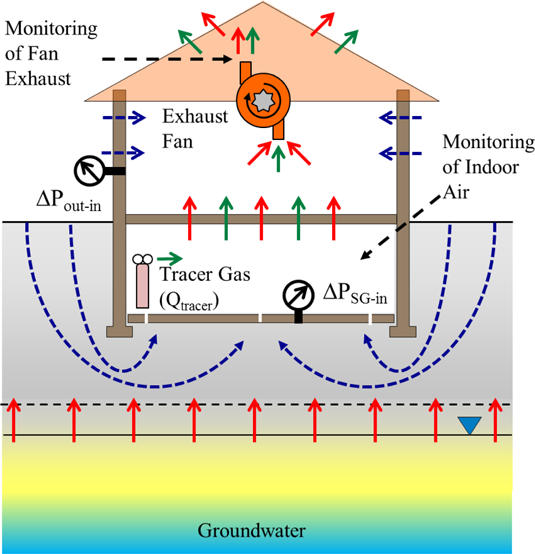
\includegraphics[width=0.75\textwidth]{cpm_cartoon.jpg}
  \caption[Overview of the controlled pressure method concept]{Conceptual idea of the controlled pressure method - a VI impacted building is forcefully pressurized using a blow, theoretically controlling the contaminant entry into the building. Figure from \citeauthor{holton_long-term_2015}\cite{holton_long-term_2015}.}
  \label{fig:cpm_cartoon}
\end{figure}

Within the CPM framework, overpressurizing a building will then prevent contaminant entry from occurring.
Thus, this can be used to identify indoor contaminant sources, as the presence of any contaminant vapors in the indoor environment in the overpressurized building have to originate from such a source.
This approach can be applied as needed and hopefully will reduce the uncertainty and difficulty of VI investigations\cite{mchugh_evaluation_2012}.\par

\subsection{Indicators, Tracers, and Surrogates}

The conventional sampling schemes currently employed, due to the spatial and temporal variability of VI, has a propensity for creating false positives and negatives.
While one solution to this problem is to increase the scope of VI investigations of a particular site, by for instance continuously monitoring the indoor contaminant concentration or by collecting an increasing number of samples, this approach is not practical, especially when numerous sites are involved.
Thus, there is a need to develop guidelines that help reduce the sampling requirements and scope of VI investigations, while retaining the same degree of confidence that the relevant level of VI has been determined\cite{schuver_chlorinated_2018}.\par

To achieve this, it has been suggested to use indicators, surrogates, and tracers (ITS) to determine when to conduct a VI site investigation.
For example, one question that has been posed is if meteorological ITS be used to determine when VI is expected to be the greatest, e.g. at which temperature and barometric pressure is, for instance, the \nth{95} percentile indoor contaminant concentration most likely to be found\cite{schuver_chlorinated_2018}?
This is a promising approach, because as we have already discussed, many VI sites have the highest indoor contaminant concentration during colder seasons.
So far this is more of a qualitative observation rather than quantitative guidelines for use in VI site investigations.\par

\begin{comment}
Main point is to point the issues with manipulating or utilizing an external variable.
I.e. sites give different responses to the same stimuli.
Again present a few examples of this (maybe just one?), but perhaps quite short as this will be covered in more detail in subsequent chapters.

Present thesis at the end of this section? (Probably)

Thesis:

Manipulation or use of external variables in VI will not yield the desired outcome, unless we improve our physical or mechanistic understanding of how these variables affect contaminant transport (or other phenomena).

Specifically, considering or determining the nature of the contaminant transport, whether advective or diffusive transport dominates, as it is key for understanding why different sites respond so differently to a change in pressurization.

For example, if contaminant transport is dominated diffusion, almost no relationship between entry rate and pressurization will exist, and as such pressurization might be a poor ITS, or CPM might not be as effective at such a site.

On the other hand, if advective transport dominates, pressurization can be a great ITS as advective transport is driven to a large degree by a pressure gradient.
\end{comment}

\section{Issues With Applying CPM \& Using ITS} % TODO: Improve title

On the surface, the CPM and ITS methods are two different approaches that tries to alleviate the same problem.
However, they both attempt to utilize some external variable, such as building pressurization, and either manipulate it directly, or by inference, to determine or predict the indoor contaminant concentration.

The issue with these approaches is that it assumes that different VI sites will respond comparably to these external variables, which in reality is not the case.
\citeauthor{guo_identification_2015}\cite{guo_identification_2015} used CPM to (inadvertently) identify a preferential pathway at their site, closed it, and noticed a markedly different relationship between indoor contaminant concentration and building pressurization for the period before and after the closing of the preferential pathway.\par % TODO: Add reference to preferential pathway chapter

The reason for this change in behavior will be elaborated on in Chapter (TBD), but consider that contaminant transport occurs through two means - diffusion and advection. % TODO: Chapter reference
If advective transport dominates, then one would expect a strong correlation between building pressurization and contaminant entry rate, which in turn largely determines the indoor contaminant concentration; if diffusive transport dominates, this relationship would be absent or weak.\par

Thus, to reliably apply any techniques such as CPM or the use of ITS, one needs a good mechanistic understanding of how, for instance, contaminant transport occurs at a VI site, and how the various site specific characteristics give rise to different transport phenomena.
Achieving this in the field can be challenging, and therefore we turn to the use of numerical models of VI scenarios from a first-principles perspective, which gives the ability to study physical phenomena in great detail.\par

\section{Modeling A Preferential Pathway}

To investigate the role a land drain type preferential pathway may have on a VI site, we extend the VI model presented in Chapter \ref{chp:method}.
By adding a gravel sub-base layer underneath the foundation slab and a preferential pathway to this model, we develop a VI model scenario that is similar to the ASU house.\par

Here we assume the gravel sub-base layer is \SI{30}{\centi\metre} thick and extends from the edges of the foundation slab.
While the exact thickness of the gravel sub-base layer at the ASU house is not known, it was estimated to be roughly that thick.
The soil surrounding the house is assumed to be homogenous sandy clay.
This is based on a description of the soil, and was chosen as the most appropriate choice is some modeling work  by \citeauthor{guo_vapor_2015}\cite{guo_vapor_2015}, one of the researchers at the ASU house.\par

The gravel sub-base, unlike the rest of the soil, is going to be relatively dry; it is covered by the foundation slab, so no rain infiltration will occur and due to the coarseness of the gravel, no moisture will be drawn up by capillary force.
Nonetheless, some van Genuchten parameters for the gravel are necessary to solve the model.
Additionally, based on the site description, we will assume that the surrounding soil is sandy clay, a , one of the researchers at the ASU house.
Table \ref{tbl:soils} has the van Genuchten parameters used to model these.\par

\begin{figure}[hbt!]
  \centering
  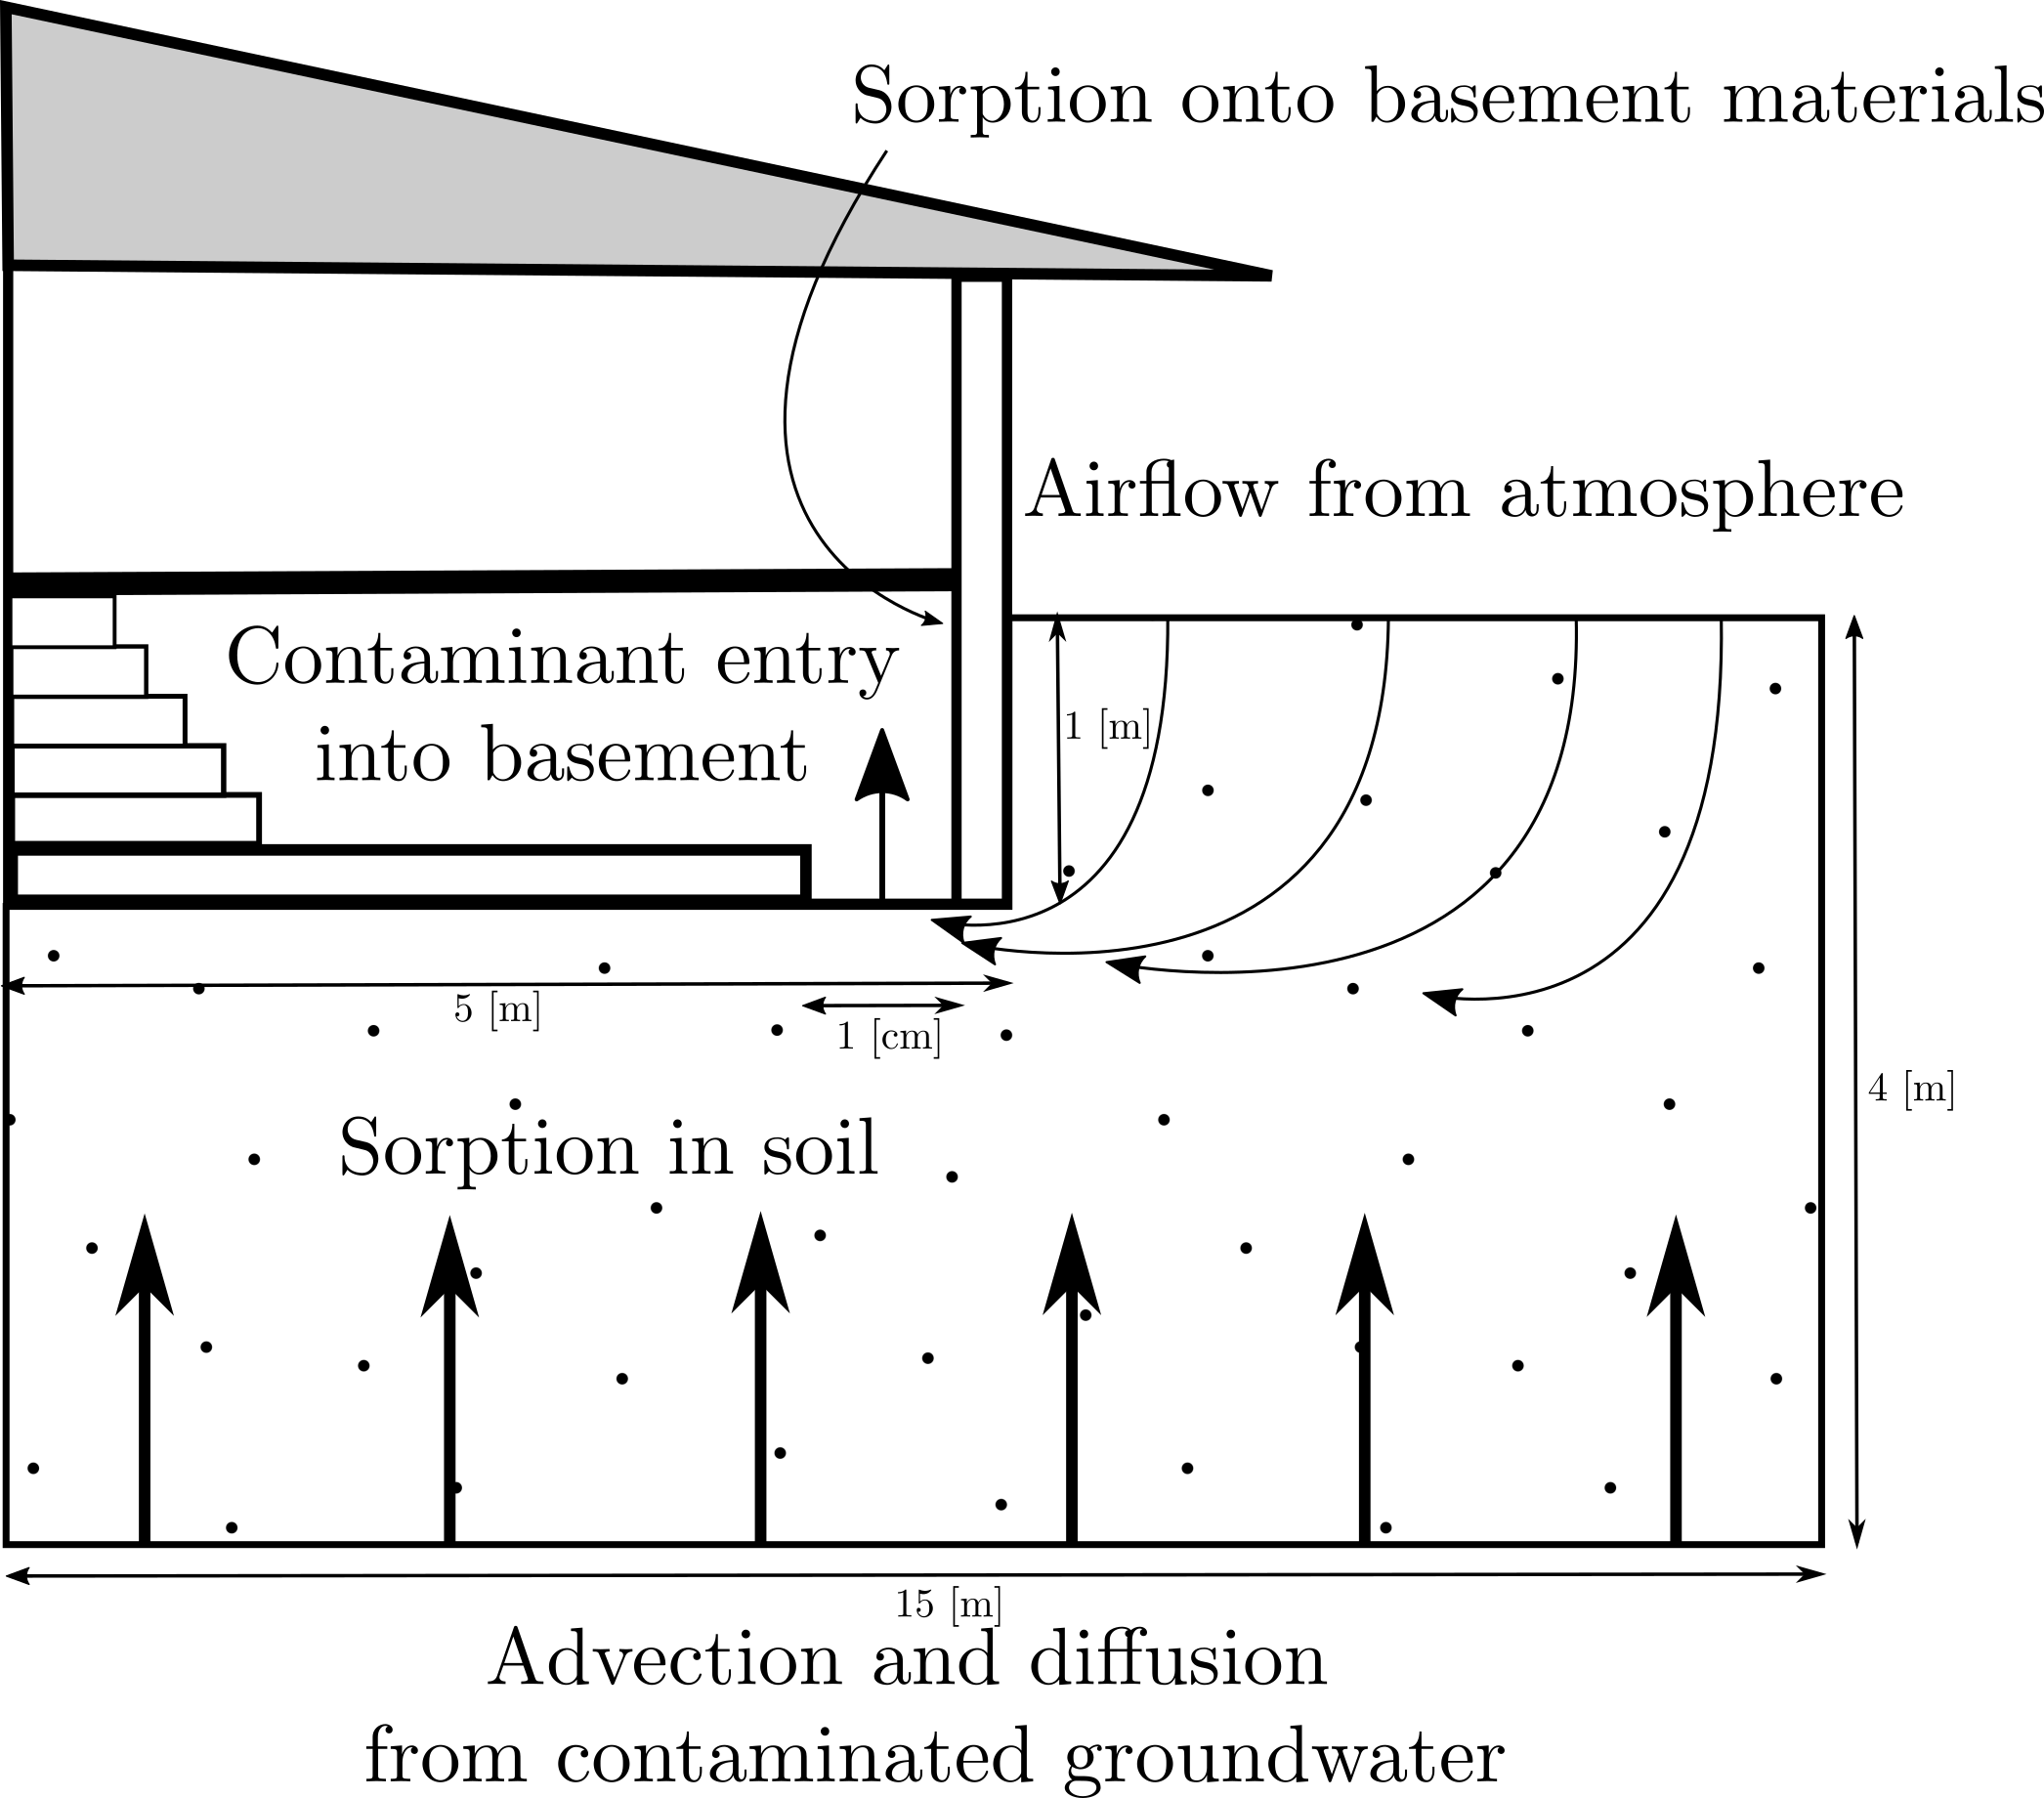
\includegraphics[width=0.75\textwidth]{model.png}
  \caption{The modeled preferential pathway VI scenario.}
  \label{fig:model_preferential_pathway}
\end{figure}

Based on the description of the land drain preferential pathway at the ASU site, we will model a preferential pathway as \SI{10}{\centi\metre} diameter pipe that exits at the interface between the soil and gravel sub-base layer; placing it near the foundation crack - similar to the ASU house\cite{guo_identification_2015}.
Figure \ref{fig:model_preferential_pathway} shows the described scenario.\par


\subsection{Geometry And Mesh}

Explicitly modeling the entire preferential pathway in detail would requires a significant number of elements and at little gain; contaminant vapor transport in the far corners of the model are not of great interest.
To save computational resources only the exit of the pipe is modeled as a \SI{10}{\centi\metre} diameter circle.\par

The existence of the preferential pathway pipe circle, only one plane of symmetry exists instead of two, and half of the model geometry has to be explicitly constructed instead of just a quarter like in Chapter \ref{chp:method}.\par

The meshing of the model follows the steps detailed in Chapter \ref{chp:method}, with the exception that a boundary layer mesh generated on the preferential pathway circle; a similar initial mesh is generated with subsequent adaptive mesh refinement.
Figure \ref{fig:model_meshed} shows the resulting meshed geometry.\par

% TODO Add mesh information in the description.
% TODO Get an image of the adapted mesh, or is this it?
\begin{figure}[htb!]
  \centering
  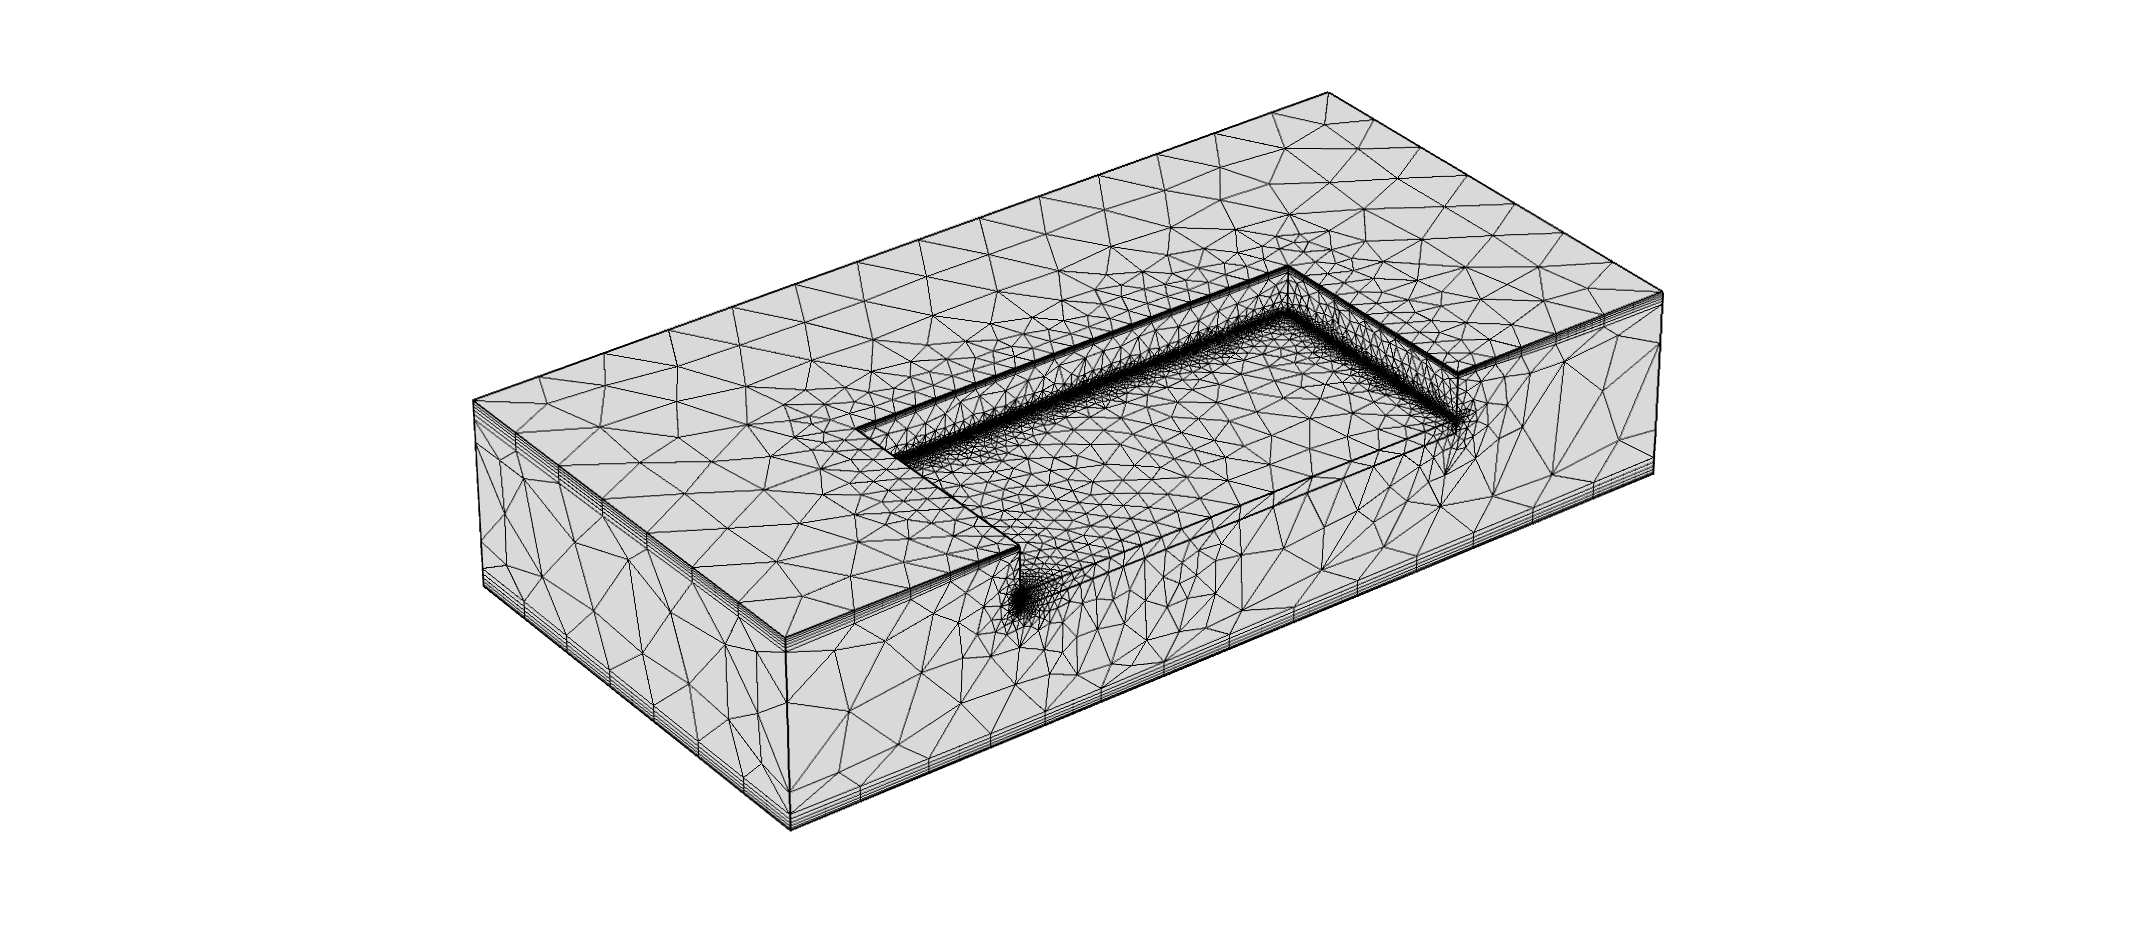
\includegraphics[width=0.75\textwidth]{model_meshed.png}
  \caption{Meshed geometry of the preferential pathway model. Notice the gravel sub-base layer and the preferential pathway exit.}
  \label{fig:model_meshed}
\end{figure}

\subsection{Physics And Boundary Conditions}

In this model, we use the same governing equations introduced in Chapter \ref{chp:method}, but are included here for completeness.
However, to simulate the preferential pathway, we will need to supply two new boundary conditions  - one for the airflow in the soil governed by Darcy's Law, and another for the soil contaminant transport, which are discussed in their respective section below.

\subsubsection{Indoor Environment}

The indoor environment is modeled using:
\begin{align*}
    V_\mathrm{bldg}\frac{\partial c_\mathrm{in}}{\partial t} &= n_\mathrm{ck} - V_\mathrm{bldg} A_e c_\mathrm{in} \\
    n_\mathrm{ck} &= \int_{A_\mathrm{ck}} j_\mathrm{ck} dA \\
    j_{ck} &= \begin{cases}
      u_{ck} c_g - \frac{D_\mathrm{air}}{L_\mathrm{slab}} (c_{in} - c_g) & u_{ck} \geq 0 \\
      u_{ck} c_{in} - \frac{D_\mathrm{air}}{L_\mathrm{slab}} (c_{in} - c_g) & u_{ck} < 0
  \end{cases}
\end{align*}
$c_\mathrm{in}$ [\si{\mol\per\metre\cubed}] is the indoor contaminant concentration;
$n_\mathrm{ck}$ [\si{\mol\per\second}] is the contaminant entry rate into the building via the foundation crack;
$A_\mathrm{ck}$ [\si{\metre\squared}] is the foundation crack boundary area;
$A_e = \SI{0.5}{\per\hour}$ is the air exchange rate;
$V_\mathrm{bldg} = \SI{300}{\metre\cubed}$ is the volume of the house basement.
$D_\mathrm{air} = \SI{7.2e-6}{\metre\squared\per\second}$ is the diffusion coefficient of TCE in air;
$u_{ck}$ [\si{\metre\per\second}] is the airflow velocity through the foundation crack;
$L_\mathrm{slab} = \SI{15}{\centi\metre}$ is the thickness of the foundation slab;
and $c_g$ [\si{\mol\per\metre\cubed}] is the contaminant gas-phase concentration at the foundation crack boundary.\par

\subsubsection{Soil Moisture}

Soil moisture content is determined using van Genuchten's retention model.
We use two "soil" types in this model - gravel and sandy clay; their parameters and constants are shown in Table \ref{tbl:soils} in the appendix.
\begin{align*}
  \mathrm{Se} &=
    \begin{cases}
      \frac{1}{(1 + (\alpha |h|)^n)^m} & \quad\quad\quad\quad\quad\quad h < 0 \\
    1 & \quad\quad\quad\quad\quad\quad h \geq 0
    \end{cases}\\
  \theta_w &=
    \begin{cases}
      \theta_r + \mathrm{Se}(\theta_t - \theta_r) & \quad\quad\quad\quad h < 0 \\
      \theta_t & \quad\quad\quad\quad h \geq 0
    \end{cases}\\
    k_r &= \begin{cases}
        \mathrm{Se}^l \big[ 1 - \big( 1 - \mathrm{Se}^\frac{1}{m} \big) \big]^2 & \quad\quad h < 0 \\
        0 & \quad\quad h \geq 0
      \end{cases}\\
    \theta_g &= \theta_t - \theta_w
\end{align*}
$h$ [\si{\metre}] is the elevation above the groundwater interface;
$\mathrm{Se}$ is the saturation;
$\alpha$, $m$, $n=\frac{1}{1-m}$, $l=0.5$ are the van Genuchten parameters;
$\theta_w$ is the water filled porosity;
$\theta_g$ is the gas filled pororsity;
$\theta_t$ is the soil porosity;
$\theta_r$ is the residual moisture content.
and $k_r$ is the relative permeability for water;

\subsubsection{Soil Airflow}

Airflow is modeled using our modified Darcy's Law expression.
\begin{equation*}
  \frac{\partial}{\partial t} (\rho \theta_g) + \nabla \cdot \rho \Big( -\frac{(1-k_r) \kappa}{\mu} \nabla p \Big) = 0
\end{equation*}
$\vec{u}$ [\si{\m\per\second}] is the airflow velocity vector;
$\kappa$ [\si{\metre\squared}] is the permeability of the porous medium;
$\mu$ [\si{\pascal\second}] is the dynamic viscosity of the fluid;
$\nabla p$ [\si{\pascal\per\metre}] is the pressure gradient;
$\theta_g$ is the gas-filled porosity of the soil;
$\rho = \SI{1.225}{\kilogram\per\metre\cubed}$ is the density of air;
and $\mu = \SI{18.5e-6}{\pascal\second}$ is the dynamic viscosity of air.\par

\paragraph{Boundary conditions}

Since the preferential pathway is assumed to be an open pipe, we assume it acts like a pressure gauge, just like the atmosphere, and is at the reference ambient atmospheric pressure.
\begin{align*}
    &\text{Ground surface} &p = \SI{0}{\pascal} \\
    &\text{Preferential pathway} &p = \SI{0}{\pascal} \\
    &\text{Foundation crack} &p = p_\mathrm{in/out} \; \si{\pascal} \\
    &\text{Remaining} &-\vec{n}\cdot\rho\vec{u} = 0
\end{align*}
$p_\mathrm{in/out}$ is not specified here as we will parametrically choose values for it.\par

\subsubsection{Soil Contaminant Transport}

The contaminant transport in the soil is governed by:
\begin{equation*}
  (\theta_w + \theta_g K_H) \frac{\partial c_w}{\partial t} = \nabla \cdot (D_\mathrm{eff} \nabla c_w) - K_H \vec{u}_g \cdot \nabla c_w
\end{equation*}
$c_w$ and $c_g$ [\si{\mol\per\metre\cubed}] are the contaminant concentrations in water and gas respectively;
$K_H = 0.402$ is the dimensionless Henry's Law constant for TCE at \SI{20}{\degreeCelsius};
$\vec{u}_g$ [\si{\metre\per\second}] is the Darcy's velocity field;
and $D_\mathrm{eff}$ [\si{\metre\squared\per\second}] is the effective diffusivity of the contaminant according to Millington-Quirks model:
\begin{equation*}
  D_\mathrm{eff} = \Big(D_w \frac{\theta_w^{\frac{10}{3}}}{\theta_t^2} + D_g \frac{\theta_g^{\frac{10}{3}}}{\theta_t^2} K_H\Big)
\end{equation*}
$D_w = \SI{1.02e-9}{\metre\squared\per\second}$ and $D_g = \SI{6.87e-6}{\metre\squared\per\second}$ are the diffusion coefficient of TCE in water and air respectively;

\paragraph{Boundary conditions}

The air in the pipe is assumed to be contaminated with TCE at a vapor concentration equal to the vapor in equilibrium with the groundwater source contaminant concentration.
This assumption is based on contaminant samples taken from a manhole near the ASU house\cite{guo_vapor_2015} which demonstrated that contaminant vapor concentrations in the nearby sewer were on similar magnitude as near the contaminated groundwater source.
\begin{align*}
  &\text{Atmosphere} & c_w = \SI{0}{\mol\per\metre\cubed} \\
  &\text{Groundwater} & c_w = c_{gw} \; \si{\mol\per\metre\cubed} \\
  &\text{Preferential pathway} & c_g = c_{gw} K_H \; \si{\mol\per\metre\cubed} \\
  &\text{Foundation crack} & -\vec{n} \cdot \vec{N} = \frac{-j_{ck}}{K_H} \; \si{\mol\per\metre\squared\per\second}\\
  &\text{All other} & -\vec{n} \cdot \vec{N} = \SI{0}{\mol\per\metre\squared\per\second}
\end{align*}
Note that we are neglecting any sorption in the soil, i.e. the sorption partitioning coefficient $K_p = \SI{0}{\metre\cubed\per\kilo\gram}$.
We will likewise normalize all concentrations to the source concentration $c_{gw}$, and any arbitrary value can be assigned.\par

\section{Outline}

Numerical models of VI scenarios will be used throughout this work, and understanding the underlying mathematics that governs VI, as well as how these models are implemented, are crucial for understanding this work.
Chapter \ref{chp:modeling} covers these aspects of VI modeling, where we develop a model of a hypothetical VI scenario.
Here, the governing equations will be introduced, as well as the finite element method (FEM), which will be used to solve our model.
In this process, we will cover the work of constructing a model geometry mesh, configuring solvers, post-processing results, and a variety of practical considerations when modeling VI.
Lastly, a brief summary of VI models and recent developments will be addressed.\par

With this knowledge of VI modeling, we will first use them to tackle the issues of preferential pathways in Chapter \ref{chp:preferential_pathways}.
A significant focus is  placed on modeling and analyzing the preferential pathway found at the "ASU house" VI site in Layton, Utah.
This work will demonstrate how and why preferential pathways can contribute so greatly to temporal and spatial variability in VI.
The preferential pathway at "EPA duplex" VI site in Indianapolis, Indiana, will also be explored here.\par

From the work in Chapter \ref{chp:preferential_pathways}, we find that it is important to consider if vapor contaminant transport from the subsurface into a building is dominated by advective or diffusive transport, a topic that will be further explored in Chapter \ref{chp:transport_implications}.
Here we discuss some of the site specific conditions that give rise to either of these transport mechanisms to dominate.
These conclusions have wider implications for CPM or using ITS, and the efficacy of these investigative methods can hinge on characterizing the dominant transport mechanism at a site.
We also explore how weather conditions and outdoor temperature can be used to predict building pressurization, which becomes an important potential ITS for advection dominated sites.\par

In Chapter \ref{chp:sorption} the role that sorption of vapor contaminant in the indoor environment and onto soil particles is explored.
The capacity of a variety of common materials to sorb TCE are measured at relevant conditions, where we find that these capacities can vary by orders of magnitude.
These sorption data are then applied to a VI model, where the potential influence of these sorption effects on contaminant transport, VI investigations, and application of mitigation systems.\par

Lastly, Chapter \ref{chp:future_work} provides a summary of the conclusions and findings in this thesis, and suggestions future work.\par


\section{Indoor Air Quality and Vapor Intrusion}
% History and perspective on indoor air quality
Concerns about air quality are as old as civilization itself, ranging from beliefs that disease is caused by bad air - a \textit{miasma}, to more recent concerns about exposure to combustion particulates, radon gas, or other air-borne pollutants.
Since industrialization the number of potential hazardous pollutants has increased significantly, followed by increased concerns about air quality.
At the same time, people now spend more time indoors now than ever before, with Americans spending up to 90\% of their waking time indoors\cite{klepeis_national_2001}.
This change in human habitation has put a special emphasis on indoor air quality.\par

Some early scientific inquiries into indoor air quality focused on pollutant sources that were generated in the home, e.g. by heating and cooking systems, and these types of pollutants are still relevant today, but of particular concern in developing countries\cite{craig_d._hollowell_combustion-generated_1976,world_health_organisation_who_2014}.
Many buildings materials can also cause indoor air quality issues, with exposure to asbestos fibers being perhaps one of the more famous examples of this.
Mold is another common indoor quality concern\cite{world_health_organisation_who_2009}.\par

% Introducing Rn
In the 1970s, to address the growing public health concerns, research began into the potential exposure to radioactive radon gas in buildings.
Radon gas, which is generated by the decay of naturally occurring uranium in soils and rocks, was found to be able to enter overlying building and expose the inhabitants.
This phenomena came to the public attention in the mid 1980s, after a Pennsylvanian nuclear power plant worker set off radioactivity sensors at the plant, the actual cause of which was the high concentration of radon gas in the workers home\cite{noauthor_health_nodate}.
Exposure to radon gas can significantly increase the risk of developing lung cancer, and is to this day the second leading cause of lung cancer in many countries\cite{gaskin_janet_global_nodate}.
With the discovery of radon intrusion into buildings, it did not take long for the same concerns to be extended to the entry of anthropogenic contaminant vapors - vapor intrusion (VI).\par

Vapor intrusion is the migration of contaminant vapors from a contaminant source, often contaminated groundwater, into the overlying buildings.
These vapors evaporate from the contaminated groundwater and enter through cracks in the building foundation, gaps between walls and floors, sump pits, or other openings\cite{u.s._environmental_protection_agency_oswer_2015}.
In these aspects, VI is more or less similar to radon intrusion, and thus much of the early VI research was heavily influenced by the work done by radon intrusion researchers.
This is largely true to this day, but vapor intrusion differs in some non-trivial ways, that make it an unique issue.
Many of these differences stem from the properties of the contaminants themselves, and from the fact that many of the VI contaminants that we concern ourselves with, mainly volatile organic compounds (VOCs) and chlorinated solvents, are of anthropogenic origins.\par

One difference is that radon is unstable, and has a half-life of around 3.8 days (at least Rn\textsuperscript{222}, the only naturally occurring isotope of radon), and it follows that radon accumulation will be naturally mitigated, which is not the case with other contaminants\cite{schumacher_fluctuation_2012}.
The closest analogy is that certain VOCs of VI concern are able to be biodegraded by bacteria in the soil, but this effect can vary significantly as this process is oxygen limited\cite{u.s._environmental_protection_agency_oswer_2015,abreu_simulating_2006}.\par

A more significant difference is the anthropogenic origin of VI contaminants.
In VI, we often are concerned with a contaminated groundwater source underneath the afflicted building, and the source of the groundwater contamination typically originates from some contaminant spill at one or more sites in the surrounding area.
Thus, a large number of buildings may be impacted by VI via a single contaminant source.
The origins of such spills are numerous, but any activities that employ the contaminants of VI concern are possible culprits\cite{u.s._environmental_protection_agency_oswer_2015}.
In the United States (US), the Environmental Protection Agency (EPA) maintains a list of significantly polluted sites throughout the country, so called Superfund sites, and as of 2020 there are 1335 recorded sites, many of which contain the contaminants of concern\cite{us_epa_current_2015,u.s._environmental_protection_agency_oswer_2015}.
Additionally, many of the contaminants of concern do not readily degrade, and legacy contamination is an issue\cite{u.s._environmental_protection_agency_oswer_2015}.
It should also be noted that VI from a contaminated groundwater is only one type of contaminant source, with leaky subsurface tanks, spills into soils, etc., likewise being contaminant sources of concern.
Figure \ref{fig:vapor_intrusion} shows some of the VI processes.\par

\begin{figure}[htb!]
  \centering
  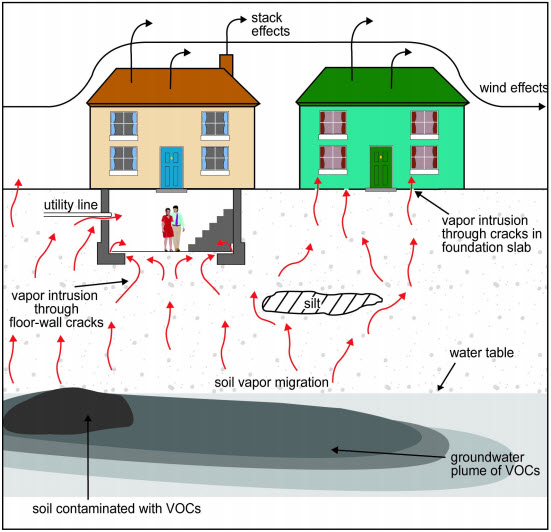
\includegraphics[width=0.75\textwidth]{vaporintrusion.jpg}
  \caption[Overview of vapor intrusion]{Vapor intrusion into a building can occur through a variety of means, from a variety of sources. Figure from the EPA\cite{us_epa_what_2015}.}
  \label{fig:vapor_intrusion}
\end{figure}

In VI, some common contaminants of concern are chlorinated solvents such as trichloroethylene (TCE), tetrachloroethylene (PCE), or chloroform.
Various other organic compounds such as benzene, or other petroleum products are also of concern.
Out of the various VI contaminants, TCE has emerged as of perhaps particular concern.
TCE is an excellent degreaser and has seen extensive use as such, and has been commonly used by dry cleaners, the military, auto repair shops etc\cite{u.s._environmental_protection_agency_oswer_2015}.
The concern over TCE is partly due to its associated cancer risk and partly because it was recently hypothesized to possibly play a role in birth defects.
A review study by \citeauthor{makris_systematic_2016}\cite{makris_systematic_2016} showed that TCE may be associated with increased risk of congenital heart defects (CHD), but a more recent study by \citeauthor{urban_systematic_2020}\cite{urban_systematic_2020} concluded that, mainly due to reproducibility issues and new studies, there is not adequate evidence to support that TCE causes CHD.
Regardless, it is carcinogenic and surprisingly despite the concerns about its health effects, its use remains legal.\par

Considering the widespread existence of potential VI sites and the associated health concerns, an industry for identifying and characterizing these sites and either remediating or mitigating them has emerged.
This is particularly true in the US, where the law dictates that the responsible party of the contaminant spill or release is liable for cleanup and mitigating human exposure.
In this situation significant effort is spent on determining liability.
Determining if VI occurs at a particular site, as we will see in this work, is not easy, and while VI has been studied for decades, many questions and challenges remain, in particular with regards to the great spatial and temporal variability that exist both within and between VI sites\cite{u.s._environmental_protection_agency_oswer_2015}.\par

\begin{comment}
Purpose is to demonstrate the issues that temporal and spatial variability causes in VI site investigations, and impress upon the reader the necessity to solve these.

- State the general issues, i.e. harder to assess real human exposure, more expensive, etc.
- Give examples in the literature and describe the situation. (1-2 examples for spatial/temporal respectively should suffice.)

Topics to cover:

Issues that confound VI investigations:
* Indoor sources/false positives (problem with only indoor samples)
* Sub-surface contaminant formation by indoor (sub-surface samples)
* Groundwater samples (spatial variability & presence of contaminants here does not mean entry occurs)
* Issues with preferential pathways
  * Indie style (long distance transport of contaminants)
  * Kelly style (plumbing fixtures)
  * ASU style (+ Danish study?) (nearby sub surface features that are not readily apparent)
* Seasonal aspect
* Necessity of MLE
  * Expensive and hard
  * Need for more robust methods

\end{comment}

\section{Issues In Vapor Intrusion Investigations}

% Some issues with VI investigations
Determining if vapor intrusion occurs at a building is often difficult.
One might be tempted to believe that collecting an indoor air sample inside the building would be sufficient, i.e. that if the vapor contaminant concentrations is over some threshold in the house, proves that IV occurs, and the absence of contaminant vapors is proof that no VI occurs.
However, this approach is too simplistic and may yield false positives.\par % TODO: Source

% False positives
Many common consumer products contain the same contaminants that is often of concern in VI, and the presence of e.g. a petroleum containing gas tank may be the culprit.
Not all indoor contaminant sources are so obvious though, and many contaminants may be inadvertently introduced, such as by bringing home newly dry-cleaned clothing.
Great care is taken to eliminate such indoor sources, but can be challenging.\par % TODO: Source

A compounding issue related to this (and other topics) is that many of the contaminants can sorb onto/into various materials and subsequently desorb for significant periods of time, potentially extending the influence of indoor source beyond their removal.
This a phenomena, among other related issues with sorption, we will discuss in Chapter (TBD).\par % TODO: Reference chapter later

Since indoor air samples may not sufficiently prove that VI occurs, one usually have to take further steps.
One such is to collect air samples right below the foundation of the building, and if contaminant vapors are found there, as well as in the indoor air, that is more compelling evidence that VI occurs.
However, as work by \citeauthor{holton_creation_2018}\cite{holton_creation_2018} has shown, contaminant vapors in the indoor environment may migrate from inside the building to the subslab, creating a contaminant cloud that may persist for significant periods of time, rendering some extra uncertainty.\par

Collecting samples from the contaminant source, such as the groundwater underneath a building, to determine the presence of contaminants can be used as another potential evidence of VI.
However, even identifying the source alone is not enough evidence as the presence of a contaminant source does not mean that the contaminant vapor enter the overlying building.
\citeauthor{folkes_observed_2009}\cite{folkes_observed_2009} who conducted a decade long study of VI sites in Redfield, Colorado, and a 19 month long study in New York showed that many of the sites, even though they were above a contaminated groundwater source, were not impacted by VI.\par

Often one would take samples from different locations, the types already discussed as well as soil-gas samples, and compare the relative decrease in contaminant vapor concentration from the source to the indoor to determine if entry ultimately occurs from the source.
This subsequent decrease is called \textit{attenuation} and is quantitively determined as an \textit{attenuation factor}, where the indoor contaminant concentration is divided by the contaminant concentration in the soil-gas or groundwater.
$\alpha$ is often used to represent the attenuation factor, and in this work we will often use a subscript to denote attenuation from where.
In the case of groundwater attenuation for instance, one would divide the indoor contaminant concentration by the groundwater contaminant vapor concentration (that is when the contaminant concentration is in equilibrium with air, e.g. Henry's Law).
\begin{equation}
  \alpha_\mathrm{gw} = \frac{c_\mathrm{in}}{c_\mathrm{gw} K_H}
\end{equation}
Where $\alpha_\mathrm{gw}$ is the attenuation from groundwater;
$c_\mathrm{in}$ i sthe indoor contaminant concentration;
$c_\mathrm{gw}$ is the groundwater \textit{liquid} contaminant concentration;
and $K_H$ is the dimensionless Henry's Law constant.\par

Over time, the U.S. Environmental Protection Agency (EPA) has compiled data of attenuation factors relative to different depths and source types.
Using these data, standards as to which attenuation factors are to be expected relative to these metrics have been established to help guide investigators and regulator determine if VI occurs.
This is helpful, but often we are faced with VI sites that render these sort of standards difficult to use.\par

Heterogeneity in soil, distribution of contaminant source concentration, as well as source type (e.g. a contaminant spill in the soil itself or some leaky chemical tank underground), can all contribute to significant spatial variability in contaminant concentration at a site.
A good example of this is a study by \citeauthor{luo_spatial_2009}\cite{luo_spatial_2009} where contaminant concentration beneath a build foundation varied from 200 to less than 0.01 mg/L.
\citeauthor{bekele_influence_2014}\cite{bekele_influence_2014} likewise found that TCE soil-gas concentration could vary an order of magnitude underneath the foundation of their site.\par

Likewise, not all indoor environments are perfectly mixed and indoor contaminant concentration can vary significantly between different rooms or compartments in a building.
This was observed at a site in Boston, Massachusetts by \citeauthor{pennell_sewer_2013}\cite{pennell_sewer_2013} who found that the indoor contaminant concentration was significantly higher in the upstairs bathroom than in the basement, where one typically would expect higher concentrations.\par

The work by \citeauthor{pennell_sewer_2013}\cite{pennell_sewer_2013} further revealed that VI could occur through sewers and enter the building through broken plumbing fixtures, which adds another level of complexity in VI - preferential pathways.
A preferential pathways is a term used describe something allows contaminant vapors to enter near or into a building, in contrast with the more "traditional" view that contaminant transport occurs through soil.
\citeauthor{mchugh_evidence_2017}\cite{mchugh_evidence_2017} studied a VI impacted building in Indianapolis, Indiana, and revealed that the sewage system there acted as a preferential pathway (in addition to the contaminated groundwater).
There contaminated groundwater infiltrated into the sewage system a few blocks away from the site, where originally an old dry cleaner had been located, and was transported to the site.\par

Similarly, \citeauthor{guo_identification_2015}\cite{guo_identification_2015} studied a site in Layton, Utah, that was found to be impacted by a sewer connected land drain that allowed contaminant vapors to be transported to the near-slab region (and close to a visible breach in the foundation).
This study and its preferential pathway is a significant focus of this work and will be discussed in more detail in Chapter (TBD).\par

\citeauthor{holton_temporal_2013}\cite{holton_temporal_2013} (same group as \citeauthor{guo_identification_2015}) demonstrated the very significant temporal variability that exist at some sites, where they found close to four orders of magnitude in variability during the multi-year study period.
\citeauthor{hosangadi_high-frequency_2017}\cite{hosangadi_high-frequency_2017} studied another site in San Diego, California, that likewise showed orders of magnitude temporal variability, albeit on a shorter time scale.
Likewise, the aforementioned site in Indianapolis had significant temporal variability\cite{schumacher_fluctuation_2012}.\par

This temporal variability often has a seasonal component, and the highest indoor contaminant concentration are usually found during the colder months of the year\cite{schumacher_fluctuation_2012,holton_temporal_2013}, although there are cases when the opposite is true. % TODO: See if you can find good source that shows VI is highest during summer
\cite{steck_indoor_2004}\cite{steck_indoor_2004} shows this at a radon impacted building in Minnesota, where the highest radon levels where observed during summer.
Some authors such as \citeauthor{bekele_influence_2014}\cite{bekele_influence_2014} suggesting that it may be necessary to collect samples at intervals across a full year, to account for all seasonal effects, to avoid mischaracterization of VI.\par

The complexity and nuances of VI has made it necessary for a multiple line-of-evidence (MLE) approach to be taken when determining if a building is impacted by VI\cite{u.s._environmental_protection_agency_oswer_2015,pennell_field_2016}.
However, the complexities associated with this necessary approach has prompted the development of new methodologies and techniques that can reduce the uncertainty and complexity associated with conducting VI site investigations.

\section{Innovations In Vapor Intrusion Investigations}

In an attempt to reduce the uncertainty in determining human exposure due to vapor intrusion caused by the significant spatial and temporal variability in VI, a number of new investigatory techniques and methods have been proposed, but in general their efficacy is yet to be fully established\cite{mchugh_recent_2017}.
This work won't deal with all of these exhaustively, but rather primarily address two approaches (together with other topics related to variability.)\par

\subsection{Controlled Pressure Method}

Most buildings are naturally depressurized relative to atmosphere due to the operation of heating, ventilation, and air conditioning systems, and the so-called stack effect, a topic that will be covered in greater detail in Chapter \ref{chp:transport_implications}.
This depressurization induces a flow of air from soil into the building; this flow can carry contaminant vapors into the building.
(This view is rather simplistic, as will be discussed throughout this work, but suffices for now.)
Using this idea, the controlled pressure method (CPM) was suggested, where blowers are used to control the depressurization of the building, and thereby more effectively control the indoor environment (see Figure \ref{fig:cpm_cartoon}).
The basic ideas was to create a "worst case" scenario in which contaminant soil vapors are induced to enter the building.\par

\begin{figure}[htb!]
  \centering
  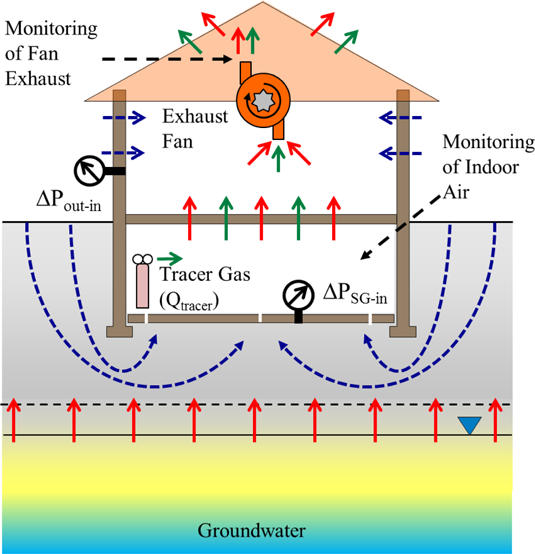
\includegraphics[width=0.75\textwidth]{cpm_cartoon.jpg}
  \caption[Overview of the controlled pressure method concept]{Conceptual idea of the controlled pressure method - a VI impacted building is forcefully pressurized using a blow, theoretically controlling the contaminant entry into the building. Figure from \citeauthor{holton_long-term_2015}\cite{holton_long-term_2015}.}
  \label{fig:cpm_cartoon}
\end{figure}

Within the CPM framework, overpressurizing a building will then prevent contaminant entry from occurring.
Thus, this can be used to identify indoor contaminant sources, as the presence of any contaminant vapors in the indoor environment in the overpressurized building have to originate from such a source.
This approach can be applied as needed and hopefully will reduce the uncertainty and difficulty of VI investigations\cite{mchugh_evaluation_2012}.\par

\subsection{Indicators, Tracers, and Surrogates}

The conventional sampling schemes currently employed, due to the spatial and temporal variability of VI, has a propensity for creating false positives and negatives.
While one solution to this problem is to increase the scope of VI investigations of a particular site, by for instance continuously monitoring the indoor contaminant concentration or by collecting an increasing number of samples, this approach is not practical, especially when numerous sites are involved.
Thus, there is a need to develop guidelines that help reduce the sampling requirements and scope of VI investigations, while retaining the same degree of confidence that the relevant level of VI has been determined\cite{schuver_chlorinated_2018}.\par

To achieve this, it has been suggested to use indicators, surrogates, and tracers (ITS) to determine when to conduct a VI site investigation.
For example, one question that has been posed is if meteorological ITS be used to determine when VI is expected to be the greatest, e.g. at which temperature and barometric pressure is, for instance, the \nth{95} percentile indoor contaminant concentration most likely to be found\cite{schuver_chlorinated_2018}?
This is a promising approach, because as we have already discussed, many VI sites have the highest indoor contaminant concentration during colder seasons.
So far this is more of a qualitative observation rather than quantitative guidelines for use in VI site investigations.\par

\begin{comment}
Main point is to point the issues with manipulating or utilizing an external variable.
I.e. sites give different responses to the same stimuli.
Again present a few examples of this (maybe just one?), but perhaps quite short as this will be covered in more detail in subsequent chapters.

Present thesis at the end of this section? (Probably)

Thesis:

Manipulation or use of external variables in VI will not yield the desired outcome, unless we improve our physical or mechanistic understanding of how these variables affect contaminant transport (or other phenomena).

Specifically, considering or determining the nature of the contaminant transport, whether advective or diffusive transport dominates, as it is key for understanding why different sites respond so differently to a change in pressurization.

For example, if contaminant transport is dominated diffusion, almost no relationship between entry rate and pressurization will exist, and as such pressurization might be a poor ITS, or CPM might not be as effective at such a site.

On the other hand, if advective transport dominates, pressurization can be a great ITS as advective transport is driven to a large degree by a pressure gradient.
\end{comment}

\section{Issues With Applying CPM \& Using ITS} % TODO: Improve title

On the surface, the CPM and ITS methods are two different approaches that tries to alleviate the same problem.
However, they both attempt to utilize some external variable, such as building pressurization, and either manipulate it directly, or by inference, to determine or predict the indoor contaminant concentration.

The issue with these approaches is that it assumes that different VI sites will respond comparably to these external variables, which in reality is not the case.
\citeauthor{guo_identification_2015}\cite{guo_identification_2015} used CPM to (inadvertently) identify a preferential pathway at their site, closed it, and noticed a markedly different relationship between indoor contaminant concentration and building pressurization for the period before and after the closing of the preferential pathway.\par % TODO: Add reference to preferential pathway chapter

The reason for this change in behavior will be elaborated on in Chapter (TBD), but consider that contaminant transport occurs through two means - diffusion and advection. % TODO: Chapter reference
If advective transport dominates, then one would expect a strong correlation between building pressurization and contaminant entry rate, which in turn largely determines the indoor contaminant concentration; if diffusive transport dominates, this relationship would be absent or weak.\par

Thus, to reliably apply any techniques such as CPM or the use of ITS, one needs a good mechanistic understanding of how, for instance, contaminant transport occurs at a VI site, and how the various site specific characteristics give rise to different transport phenomena.
Achieving this in the field can be challenging, and therefore we turn to the use of numerical models of VI scenarios from a first-principles perspective, which gives the ability to study physical phenomena in great detail.\par

\section{Modeling A Preferential Pathway}

To investigate the role a land drain type preferential pathway may have on a VI site, we extend the VI model presented in Chapter \ref{chp:method}.
By adding a gravel sub-base layer underneath the foundation slab and a preferential pathway to this model, we develop a VI model scenario that is similar to the ASU house.\par

Here we assume the gravel sub-base layer is \SI{30}{\centi\metre} thick and extends from the edges of the foundation slab.
While the exact thickness of the gravel sub-base layer at the ASU house is not known, it was estimated to be roughly that thick.
The soil surrounding the house is assumed to be homogenous sandy clay.
This is based on a description of the soil, and was chosen as the most appropriate choice is some modeling work  by \citeauthor{guo_vapor_2015}\cite{guo_vapor_2015}, one of the researchers at the ASU house.\par

The gravel sub-base, unlike the rest of the soil, is going to be relatively dry; it is covered by the foundation slab, so no rain infiltration will occur and due to the coarseness of the gravel, no moisture will be drawn up by capillary force.
Nonetheless, some van Genuchten parameters for the gravel are necessary to solve the model.
Additionally, based on the site description, we will assume that the surrounding soil is sandy clay, a , one of the researchers at the ASU house.
Table \ref{tbl:soils} has the van Genuchten parameters used to model these.\par

\begin{figure}[hbt!]
  \centering
  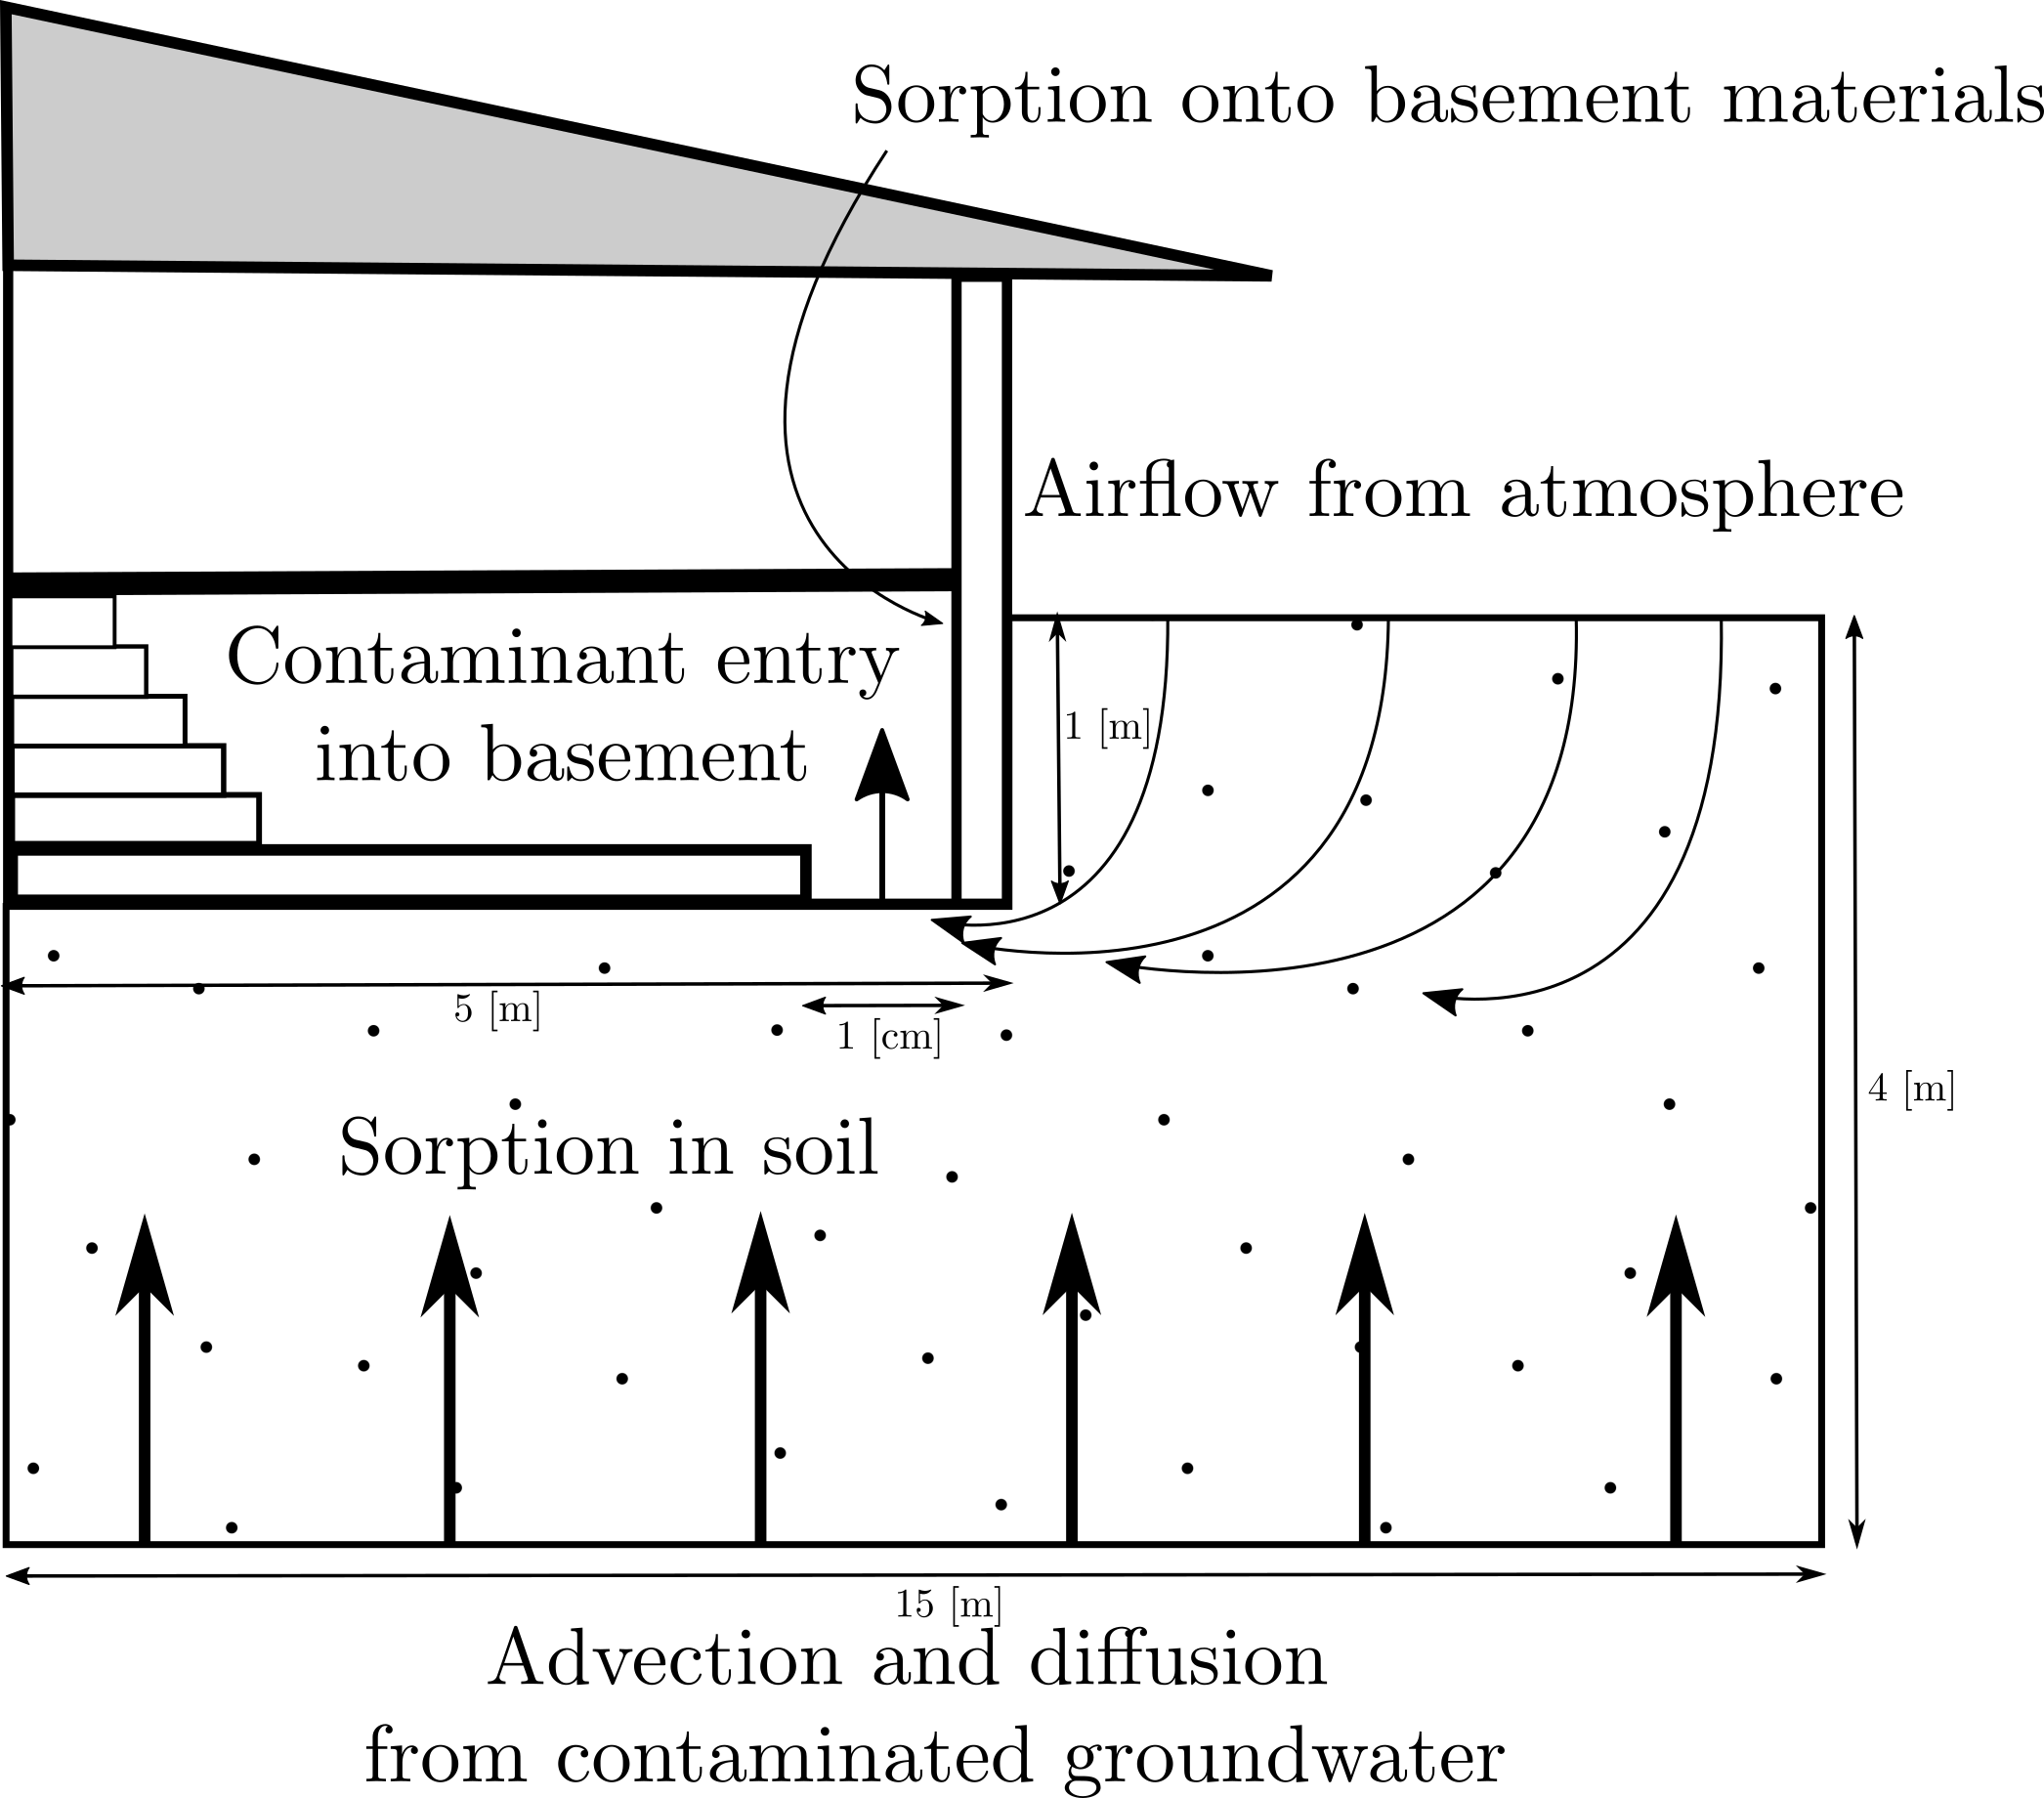
\includegraphics[width=0.75\textwidth]{model.png}
  \caption{The modeled preferential pathway VI scenario.}
  \label{fig:model_preferential_pathway}
\end{figure}

Based on the description of the land drain preferential pathway at the ASU site, we will model a preferential pathway as \SI{10}{\centi\metre} diameter pipe that exits at the interface between the soil and gravel sub-base layer; placing it near the foundation crack - similar to the ASU house\cite{guo_identification_2015}.
Figure \ref{fig:model_preferential_pathway} shows the described scenario.\par


\subsection{Geometry And Mesh}

Explicitly modeling the entire preferential pathway in detail would requires a significant number of elements and at little gain; contaminant vapor transport in the far corners of the model are not of great interest.
To save computational resources only the exit of the pipe is modeled as a \SI{10}{\centi\metre} diameter circle.\par

The existence of the preferential pathway pipe circle, only one plane of symmetry exists instead of two, and half of the model geometry has to be explicitly constructed instead of just a quarter like in Chapter \ref{chp:method}.\par

The meshing of the model follows the steps detailed in Chapter \ref{chp:method}, with the exception that a boundary layer mesh generated on the preferential pathway circle; a similar initial mesh is generated with subsequent adaptive mesh refinement.
Figure \ref{fig:model_meshed} shows the resulting meshed geometry.\par

% TODO Add mesh information in the description.
% TODO Get an image of the adapted mesh, or is this it?
\begin{figure}[htb!]
  \centering
  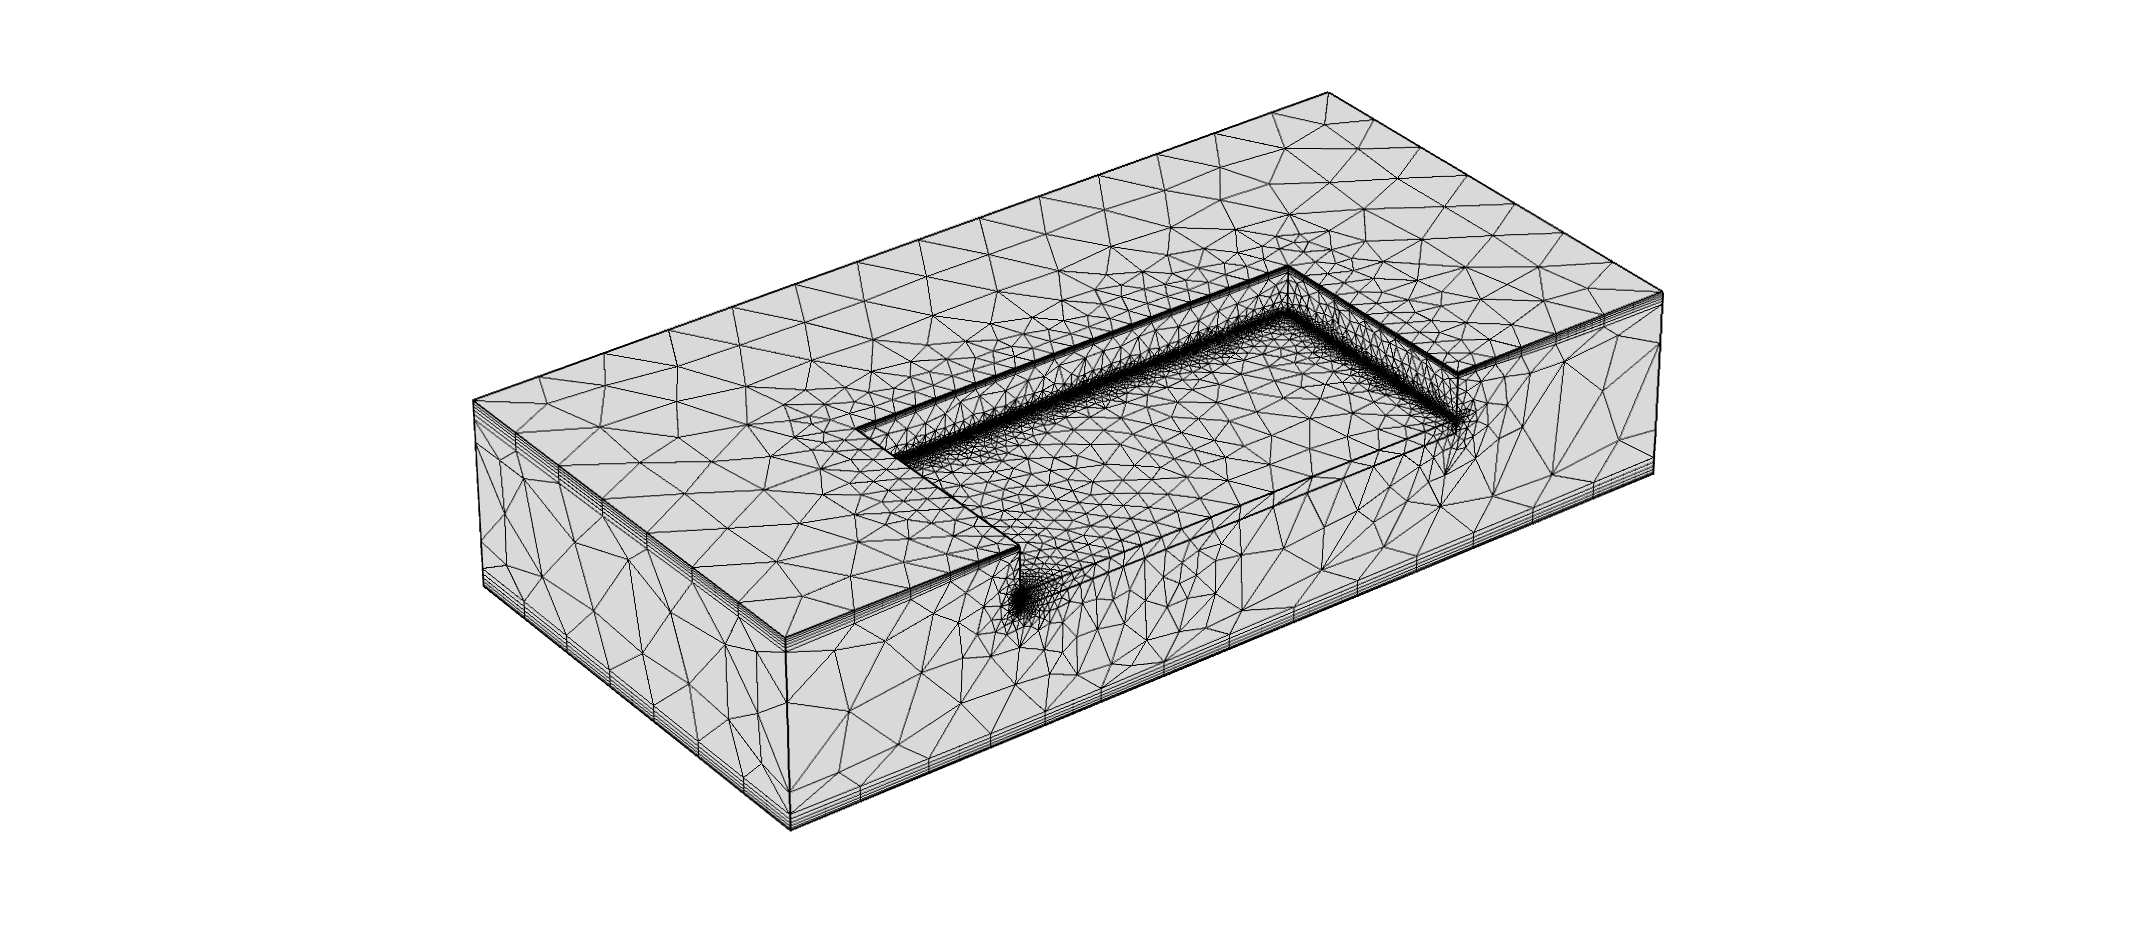
\includegraphics[width=0.75\textwidth]{model_meshed.png}
  \caption{Meshed geometry of the preferential pathway model. Notice the gravel sub-base layer and the preferential pathway exit.}
  \label{fig:model_meshed}
\end{figure}

\subsection{Physics And Boundary Conditions}

In this model, we use the same governing equations introduced in Chapter \ref{chp:method}, but are included here for completeness.
However, to simulate the preferential pathway, we will need to supply two new boundary conditions  - one for the airflow in the soil governed by Darcy's Law, and another for the soil contaminant transport, which are discussed in their respective section below.

\subsubsection{Indoor Environment}

The indoor environment is modeled using:
\begin{align*}
    V_\mathrm{bldg}\frac{\partial c_\mathrm{in}}{\partial t} &= n_\mathrm{ck} - V_\mathrm{bldg} A_e c_\mathrm{in} \\
    n_\mathrm{ck} &= \int_{A_\mathrm{ck}} j_\mathrm{ck} dA \\
    j_{ck} &= \begin{cases}
      u_{ck} c_g - \frac{D_\mathrm{air}}{L_\mathrm{slab}} (c_{in} - c_g) & u_{ck} \geq 0 \\
      u_{ck} c_{in} - \frac{D_\mathrm{air}}{L_\mathrm{slab}} (c_{in} - c_g) & u_{ck} < 0
  \end{cases}
\end{align*}
$c_\mathrm{in}$ [\si{\mol\per\metre\cubed}] is the indoor contaminant concentration;
$n_\mathrm{ck}$ [\si{\mol\per\second}] is the contaminant entry rate into the building via the foundation crack;
$A_\mathrm{ck}$ [\si{\metre\squared}] is the foundation crack boundary area;
$A_e = \SI{0.5}{\per\hour}$ is the air exchange rate;
$V_\mathrm{bldg} = \SI{300}{\metre\cubed}$ is the volume of the house basement.
$D_\mathrm{air} = \SI{7.2e-6}{\metre\squared\per\second}$ is the diffusion coefficient of TCE in air;
$u_{ck}$ [\si{\metre\per\second}] is the airflow velocity through the foundation crack;
$L_\mathrm{slab} = \SI{15}{\centi\metre}$ is the thickness of the foundation slab;
and $c_g$ [\si{\mol\per\metre\cubed}] is the contaminant gas-phase concentration at the foundation crack boundary.\par

\subsubsection{Soil Moisture}

Soil moisture content is determined using van Genuchten's retention model.
We use two "soil" types in this model - gravel and sandy clay; their parameters and constants are shown in Table \ref{tbl:soils} in the appendix.
\begin{align*}
  \mathrm{Se} &=
    \begin{cases}
      \frac{1}{(1 + (\alpha |h|)^n)^m} & \quad\quad\quad\quad\quad\quad h < 0 \\
    1 & \quad\quad\quad\quad\quad\quad h \geq 0
    \end{cases}\\
  \theta_w &=
    \begin{cases}
      \theta_r + \mathrm{Se}(\theta_t - \theta_r) & \quad\quad\quad\quad h < 0 \\
      \theta_t & \quad\quad\quad\quad h \geq 0
    \end{cases}\\
    k_r &= \begin{cases}
        \mathrm{Se}^l \big[ 1 - \big( 1 - \mathrm{Se}^\frac{1}{m} \big) \big]^2 & \quad\quad h < 0 \\
        0 & \quad\quad h \geq 0
      \end{cases}\\
    \theta_g &= \theta_t - \theta_w
\end{align*}
$h$ [\si{\metre}] is the elevation above the groundwater interface;
$\mathrm{Se}$ is the saturation;
$\alpha$, $m$, $n=\frac{1}{1-m}$, $l=0.5$ are the van Genuchten parameters;
$\theta_w$ is the water filled porosity;
$\theta_g$ is the gas filled pororsity;
$\theta_t$ is the soil porosity;
$\theta_r$ is the residual moisture content.
and $k_r$ is the relative permeability for water;

\subsubsection{Soil Airflow}

Airflow is modeled using our modified Darcy's Law expression.
\begin{equation*}
  \frac{\partial}{\partial t} (\rho \theta_g) + \nabla \cdot \rho \Big( -\frac{(1-k_r) \kappa}{\mu} \nabla p \Big) = 0
\end{equation*}
$\vec{u}$ [\si{\m\per\second}] is the airflow velocity vector;
$\kappa$ [\si{\metre\squared}] is the permeability of the porous medium;
$\mu$ [\si{\pascal\second}] is the dynamic viscosity of the fluid;
$\nabla p$ [\si{\pascal\per\metre}] is the pressure gradient;
$\theta_g$ is the gas-filled porosity of the soil;
$\rho = \SI{1.225}{\kilogram\per\metre\cubed}$ is the density of air;
and $\mu = \SI{18.5e-6}{\pascal\second}$ is the dynamic viscosity of air.\par

\paragraph{Boundary conditions}

Since the preferential pathway is assumed to be an open pipe, we assume it acts like a pressure gauge, just like the atmosphere, and is at the reference ambient atmospheric pressure.
\begin{align*}
    &\text{Ground surface} &p = \SI{0}{\pascal} \\
    &\text{Preferential pathway} &p = \SI{0}{\pascal} \\
    &\text{Foundation crack} &p = p_\mathrm{in/out} \; \si{\pascal} \\
    &\text{Remaining} &-\vec{n}\cdot\rho\vec{u} = 0
\end{align*}
$p_\mathrm{in/out}$ is not specified here as we will parametrically choose values for it.\par

\subsubsection{Soil Contaminant Transport}

The contaminant transport in the soil is governed by:
\begin{equation*}
  (\theta_w + \theta_g K_H) \frac{\partial c_w}{\partial t} = \nabla \cdot (D_\mathrm{eff} \nabla c_w) - K_H \vec{u}_g \cdot \nabla c_w
\end{equation*}
$c_w$ and $c_g$ [\si{\mol\per\metre\cubed}] are the contaminant concentrations in water and gas respectively;
$K_H = 0.402$ is the dimensionless Henry's Law constant for TCE at \SI{20}{\degreeCelsius};
$\vec{u}_g$ [\si{\metre\per\second}] is the Darcy's velocity field;
and $D_\mathrm{eff}$ [\si{\metre\squared\per\second}] is the effective diffusivity of the contaminant according to Millington-Quirks model:
\begin{equation*}
  D_\mathrm{eff} = \Big(D_w \frac{\theta_w^{\frac{10}{3}}}{\theta_t^2} + D_g \frac{\theta_g^{\frac{10}{3}}}{\theta_t^2} K_H\Big)
\end{equation*}
$D_w = \SI{1.02e-9}{\metre\squared\per\second}$ and $D_g = \SI{6.87e-6}{\metre\squared\per\second}$ are the diffusion coefficient of TCE in water and air respectively;

\paragraph{Boundary conditions}

The air in the pipe is assumed to be contaminated with TCE at a vapor concentration equal to the vapor in equilibrium with the groundwater source contaminant concentration.
This assumption is based on contaminant samples taken from a manhole near the ASU house\cite{guo_vapor_2015} which demonstrated that contaminant vapor concentrations in the nearby sewer were on similar magnitude as near the contaminated groundwater source.
\begin{align*}
  &\text{Atmosphere} & c_w = \SI{0}{\mol\per\metre\cubed} \\
  &\text{Groundwater} & c_w = c_{gw} \; \si{\mol\per\metre\cubed} \\
  &\text{Preferential pathway} & c_g = c_{gw} K_H \; \si{\mol\per\metre\cubed} \\
  &\text{Foundation crack} & -\vec{n} \cdot \vec{N} = \frac{-j_{ck}}{K_H} \; \si{\mol\per\metre\squared\per\second}\\
  &\text{All other} & -\vec{n} \cdot \vec{N} = \SI{0}{\mol\per\metre\squared\per\second}
\end{align*}
Note that we are neglecting any sorption in the soil, i.e. the sorption partitioning coefficient $K_p = \SI{0}{\metre\cubed\per\kilo\gram}$.
We will likewise normalize all concentrations to the source concentration $c_{gw}$, and any arbitrary value can be assigned.\par

\section{Outline}

Numerical models of VI scenarios will be used throughout this work, and understanding the underlying mathematics that governs VI, as well as how these models are implemented, are crucial for understanding this work.
Chapter \ref{chp:modeling} covers these aspects of VI modeling, where we develop a model of a hypothetical VI scenario.
Here, the governing equations will be introduced, as well as the finite element method (FEM), which will be used to solve our model.
In this process, we will cover the work of constructing a model geometry mesh, configuring solvers, post-processing results, and a variety of practical considerations when modeling VI.
Lastly, a brief summary of VI models and recent developments will be addressed.\par

With this knowledge of VI modeling, we will first use them to tackle the issues of preferential pathways in Chapter \ref{chp:preferential_pathways}.
A significant focus is  placed on modeling and analyzing the preferential pathway found at the "ASU house" VI site in Layton, Utah.
This work will demonstrate how and why preferential pathways can contribute so greatly to temporal and spatial variability in VI.
The preferential pathway at "EPA duplex" VI site in Indianapolis, Indiana, will also be explored here.\par

From the work in Chapter \ref{chp:preferential_pathways}, we find that it is important to consider if vapor contaminant transport from the subsurface into a building is dominated by advective or diffusive transport, a topic that will be further explored in Chapter \ref{chp:transport_implications}.
Here we discuss some of the site specific conditions that give rise to either of these transport mechanisms to dominate.
These conclusions have wider implications for CPM or using ITS, and the efficacy of these investigative methods can hinge on characterizing the dominant transport mechanism at a site.
We also explore how weather conditions and outdoor temperature can be used to predict building pressurization, which becomes an important potential ITS for advection dominated sites.\par

In Chapter \ref{chp:sorption} the role that sorption of vapor contaminant in the indoor environment and onto soil particles is explored.
The capacity of a variety of common materials to sorb TCE are measured at relevant conditions, where we find that these capacities can vary by orders of magnitude.
These sorption data are then applied to a VI model, where the potential influence of these sorption effects on contaminant transport, VI investigations, and application of mitigation systems.\par

Lastly, Chapter \ref{chp:future_work} provides a summary of the conclusions and findings in this thesis, and suggestions future work.\par

\end{comment}


\end{document}
